%%____________________________________________________________________________||
\section{Aggregate signal regions}
\label{sec:aggregate-signal-regions}

In order to achieve sensitivity to a wide range of new physics models searches
for BSM physics typically use fine categorisations of events in the signal region.
For example, several searches for Supersymmetry (SUSY) using data from Run 2 of the LHS
used $\mathcal{O}100$ of bins \cite{susy-searches}. Recasting such searches to determine 
the impact on models not interpreted within CMS as well as generating limits will
be very time consuming. Additionally, a large number of bins used in the CMS analyses 
may not be sensitive to the model(s) the recaster is studying. 


A simple way to sufficiently simplify the categorisation is for the recaster to take only
the bins that are relevant for their model(s), however, this necessarily breaks 
the correlation scheme used by the CMS analysis (more consideration is 
given to the correlation model in Sec~{sec:simplified-likelihood}). Instead, aggregate regions
will be defined below which allow the analyzers to simplify the categorisation through
merging signal region bins while maintaining the correlation scheme used for the full analysis.
predictions while keeping the prediction separate. This information can then be given along
with the full results to allow recasters to correctly interpret any model. The results from 
the blah blah analysis are used in this section to illustrate the use of these aggregate regions
for a new physics search.

\subsection{Defining agregate regions}

For a binned analysis which control regions are used to constrain backgrounds in the signal region
(with relevant systematics) the likelihood may generally be written in two parts, splitting the signal
and control regions. To show how the aggregate regions are defined a simplified scenario 
where each signal bin contains only one background and where each control region bin is used to
predict only one signal region bin is considered below. It is trivial to see how this may
be extended to more complex scenarios. The signal region section of the likehood may be written
as a product over bins, i, as in Equation~\ref{eq:hadronicLikelihood}.

\begin{equation}
\mathcal{L}_{\mathrm{signal}}=\prod_i{\mathrm{Pois}(n_{\mathrm{signal},i} |\, b_{\mathrm{signal},i}
\times\overline{\rho}_{\mathrm{signal},i}\times{a_i} + s_{\mathrm{signal}}\times\overline{\rho}^\mathrm{s}_{\mathrm{signal},i}\times\mu)}
\label{eq:hadronicLikelihood}
\end{equation}

where $n_{\mathrm{signal},i}$ is the observation in the signal bin, $b_{\mathrm{signal},i}$
the background prediction from simulation, $\overline{\rho_{i}}$ the set of systematics
on the signal region prediction, ${a_i}$ an unconstrained parameter that will connect to the 
control region, $s_{\mathrm{sig}}$ the signal model contribution from simulation, 
$\overline{\rho}_{i,sig}$ the set of systematics on the signal contribution and $\mu$ the
unconstrained signal strength parameter.  The connection to the control region 
may be written as in Equation~\ref{eq:controlLikelihood}.

\begin{equation}
\mathcal{L}_{\mathrm{control},i}=\prod_i{\mathrm{Pois}(n_{\mathrm{control},i} |\, b_{\mathrm{control},i}
\times\overline{\rho}_{\mathrm{control}}\times{a_i} + s_{\mathrm{control}}\times\overline{\rho}^\mathrm{s}_{\mathrm{control},i}\times\mu)}
\label{eq:controlLikelihood}
\end{equation}

where parameters are as defined in Equation~\ref{eq:hadronicLikelihood} but applied in the control region. 
Here $\overline{\rho}_{\mathrm{control},i}$ contains both systematic uncertainties on the control region
and on the connection of the control to signal region. Correlation between bins in the signal
and control regions are introduced through the correlation or anticorrelation of the systematic uncertainties
contained in both $\overline{\rho}_{\mathrm{signal},i}$ and $\overline{\rho}_{\mathrm{control},i}$. For a 
more complex likelihood additional correlations are introduced when control regions are used to predict
multiple signal region bins. The overall likelihood of $\mathcal{L}_{\mathrm{signal}}\times\mathcal{L}_{\mathrm{control}}$
is then minimized with respect to $mu$,$\rho$ and $\rho_^{mathrm{s}}$. 

The likelihood for the aggregate regions may then be defined as in Equation~\ref{eq:agg-hadronicLikelihood}.

\begin{equation}
\mathcal{L}_{\mathrm{l}}=\prod_{agg}{\mathrm{Pois}(n_{\mathrm{signal},agg} |\,\sum_i^{k_{agg}}{b_{\mathrm{signal},i}
\times\overline{\rho}_{\mathrm{signal},i}\times{a_i} + s_{\mathrm{signal}}\times\overline{\rho}^\mathrm{s}_{\mathrm{signal},i}\times\mu)}}
\times\mathcal{L}_{\mathrm{control}}$
\label{eq:agg-hadronicLikelihood}
\end{equation}

where the contributions of all bins being merged are summed to provide a total background and signal
contribution to the aggregate bin. The control region section of the likelihood
is unchanged and so the correlation model for the predictions is maintained. 
The likelihood is minimized with respect to $mu$,$\rho$, $\a_i$, $\rho_^{mathrm{s}}$ as 
before. For analyses which do not include a control region explicitely in the likelihood 
the aggregation process is similar, however, in this case the parameters $a_i$ are not 
freely floating but are instead constrained according to a pdf, such as a gamma distribution, 
which encodes the uncertainty from the control region. The form of the nominal and aggregate
likelihoods are otherwise unchanged. In Section~\ref{sec:ssr-alphat} an example of the use of 
aggregate regions is shown for the \alphat analysis.

\subsection{Application of aggregate regions for the \alphat analysis}

In this section the application of aggregate regions of the \alphat analysis
using data from Run 2 of the LHC in 2016 is considered.
The strategry of the \alphat analysis is summarised in \cite{alphaT}. 
The final \nj,\nb categories and \scalht binning used for the full likelihood 
are summarised in Table~\ref{tab:binning}. These bins are further split into
$50 \GeV$ \mht bins as defined in \cite{alphaT}. The control region
predictions are inclusive in \mht but binned according to Table~\ref{tab:binning}.

\begin{table}[htb!]
  \topcaption{Summary of the lower bounds of the first and final bins
    in \scalht (the latter in parentheses) as a function of \njet and
    \nb. Intermediate \scalht bins are taken from 200,250,300,400,500,600,700,$>800\GeV$} 
  \label{tab:binning}
  \centering
  \footnotesize
  \begin{tabular}{ lrrrr }
    \hline
%    \njet                   & \multicolumn{4}{c}{\nb}                                           \\
%    \cline{2-5}
%                            & 0         & 1         & 2         & $\geq$3                       \\
    $\njet \backslash\, \nb$ & 0         & 1         & 2         & $\geq$3                       \\
    \hline
    \multicolumn{5}{l}{\bf Monojet}                                                              \\
    1                        & 200 (600) & 200 (500) & -     & -                         \\
    \multicolumn{5}{l}{\bf Asymmetric}                                                           \\
    2                        & 200 (600) & 200 (500) & 200 (400) & -                         \\
    3                        & 200 (600) & 200 (600) & 200 (500) & 200 (300)                     \\
    4                        & 200 (600) & 200 (600) & 200 (600) & 250 (400)                     \\
    $\geq$5                  & 250 (600) & 250 (600) & 250 (600) & 300 (500)                     \\
    \multicolumn{5}{l}{\bf Symmetric}                                                            \\
    2                        & 200 (800) & 200 (800) & 200 (600) & -                         \\
    3                        & 200 (800) & 250 (800) & 250 (800) & \phantom{0}-\phantom{0} (250) \\
    4                        & 300 (800) & 300 (800) & 300 (800) & 300 (800)                     \\
    $\geq$5                  & 350 (800) & 350 (800) & 350 (800) & 350 (800)                     \\
    \hline
  \end{tabular}
\end{table}

The $\mathcal{O}800$ bins provide generic sensitivity but are not optimal
for simple reinterpretation. A simplification can be made that maintains
sensitivity to a large class of models through the use of aggregate regions.
The final categories are shown in Table~\ref{tab:agg-binnning}. In addition
for each aggregate category eight exclusive \mht bins with
lower bounds $100,200,300,400,500,600,700,\ge800GeV$ are defined.

\begin{table}[tb]
  \topcaption{Aggregate region bins. The \scalht dimension is
  merged to $\geq200\GeV$, \nb to two categories of \nb = $0,1$ and $\geq2$. 
  The merged \nj~ categories are summarised in this table. Each category is
  further binned using eight \mht bins with lower bounds from $100-800\GeV$.}
  \label{tab:agg-binning}
  \centering
  \footnotesize
  \begin{tabular}{ llll }
    \hline
    \nj topology & \multicolumn{3}{l}{Merged jet categories} \\
    \hline
     & \bf Monojet & \bf Asymmetric& \bf Symmetric \\
    Monojet-like & 1 & 2 & 2                         \\
    Asymmetric high \nj& - & 3, 4, $\geq5$ & -                 \\
    Mid \nj & - &  3, 4 & -                        \\
    High \nj & - & $\geq5$ & -                     \\
    \hline
  \end{tabular}
\end{table}

The jet categories are merged to four seperate categories motivated by their sensitivity to 
different new physics topologies. For example, the Monojet-like topology is targeted towards
dark matter models and compressed spectra while the high \nj topology targets 
uncompressed gluino and squark models.
The b-jet categories are combined as $\nb=0,1$ \nb models and $\nb\geq2$ targeted at
light and heavy flavour new physics respectively. Finally, the \scalht dimension is 
entirely merged as the \mht dimension is strongly correlated with \scalht and
can be used to provide similar sensitivity. The use of the
aggregate regions ensures that the components of the background are still
corrected based on the nominal, finely binned regions with relevant systematics.

\subsection{Results using aggregate regions for the \alphat analysis}

When using the full likelihood presenting the final fit results is
a signifcant issue. The large number of bins makes understanding any possible trends,
excesses or deficits in the fit result across the signal region difficult. 
The aggregate regions can be used to rapidly find global features in the fit result as
the full picture can be summarised, in the case of the \alphat analysis, 
in eight \mht distributions as shown in Fig.~\ref{fig:aggFitResult}. These
show the predictions using the fit to the control regions only compared to 
the data observations. Post signal region fit results are shown in Appendix~\ref{app:}.

To evaluate the effect on the sensitivity the expected and observed 95\% upper limit
on the signal strength, defined as in \cite{limit-stuff}, for the full signal region 
is compared that using the aggregate regions. The limits are shown side by side
in Fig~\ref{fig:limit-planes} for three models, T2tt T2bb and T1bbbb. Where the mass
splittings are small the expected limits typically reduce by $\mathcal{O} 100\GeV$ 
compared to the full signal region for all models  

The aggregate fit result considering only the control regions, 
can be used to provide predictions and uncertainties
to allow recasters to interpret their own models. In the case of the \alphat search
this is significantly easier than recasting the full signal region. To make best use of this information, 
as will be discussed in Section~\ref{sec:simplified-likelihood}, 
the covariance matrix encoding the level of correlation between bins must also be utilised.
\clearpage
\begin{figure}[!tbhp]
    \caption{ Signal region predictions and data observations for the aggregate regions. 
    The predictions are made using a fit to the control region only. \label{fig:aggFitResult} }
  \begin{center}
    \subfigure[Monojet-like, $\nb = 0$]{ 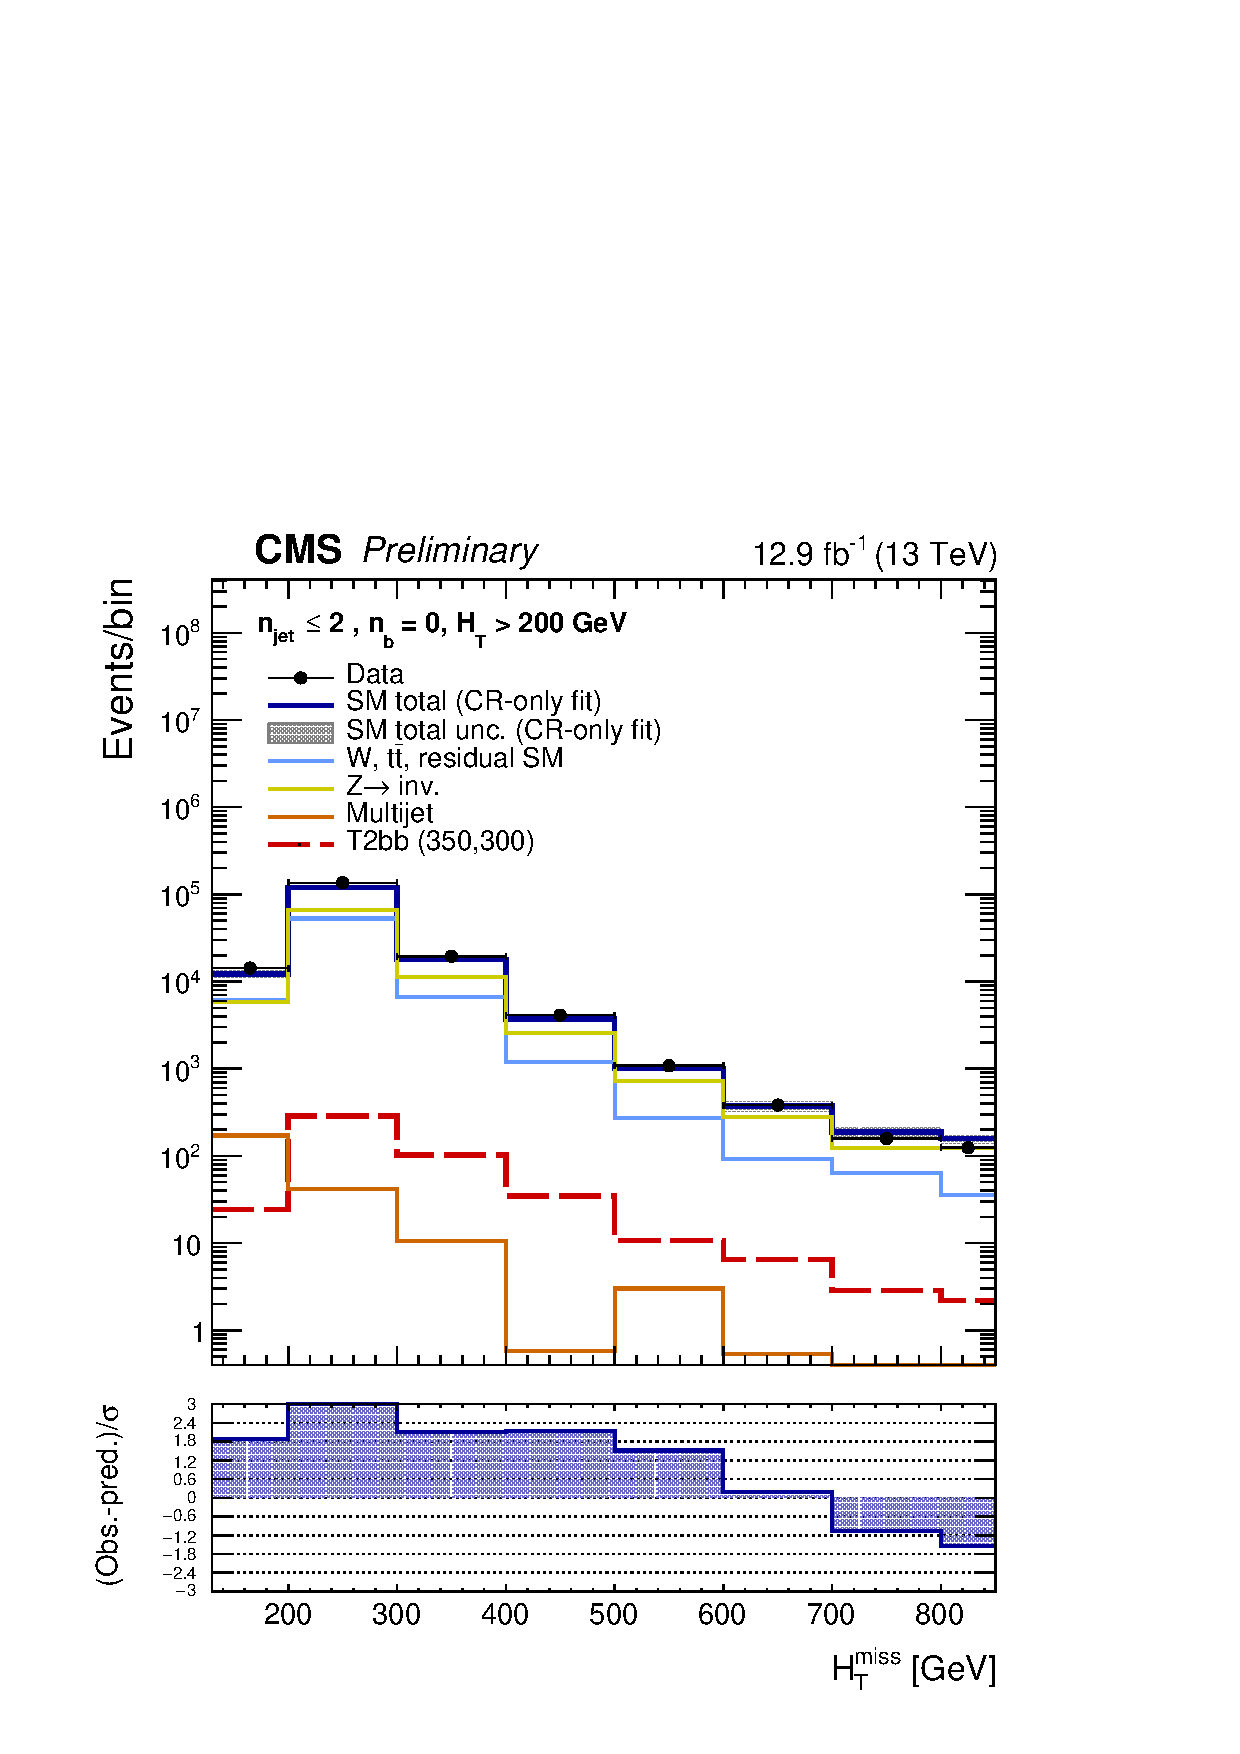
\includegraphics[width=0.4\textwidth]{figures/agg_fitResults/mhtShape_eq0b_le2j_200_Inf_crfit_aux.pdf} } ~~
    \subfigure[Monojet-like, $\nb \geq 1$]{ 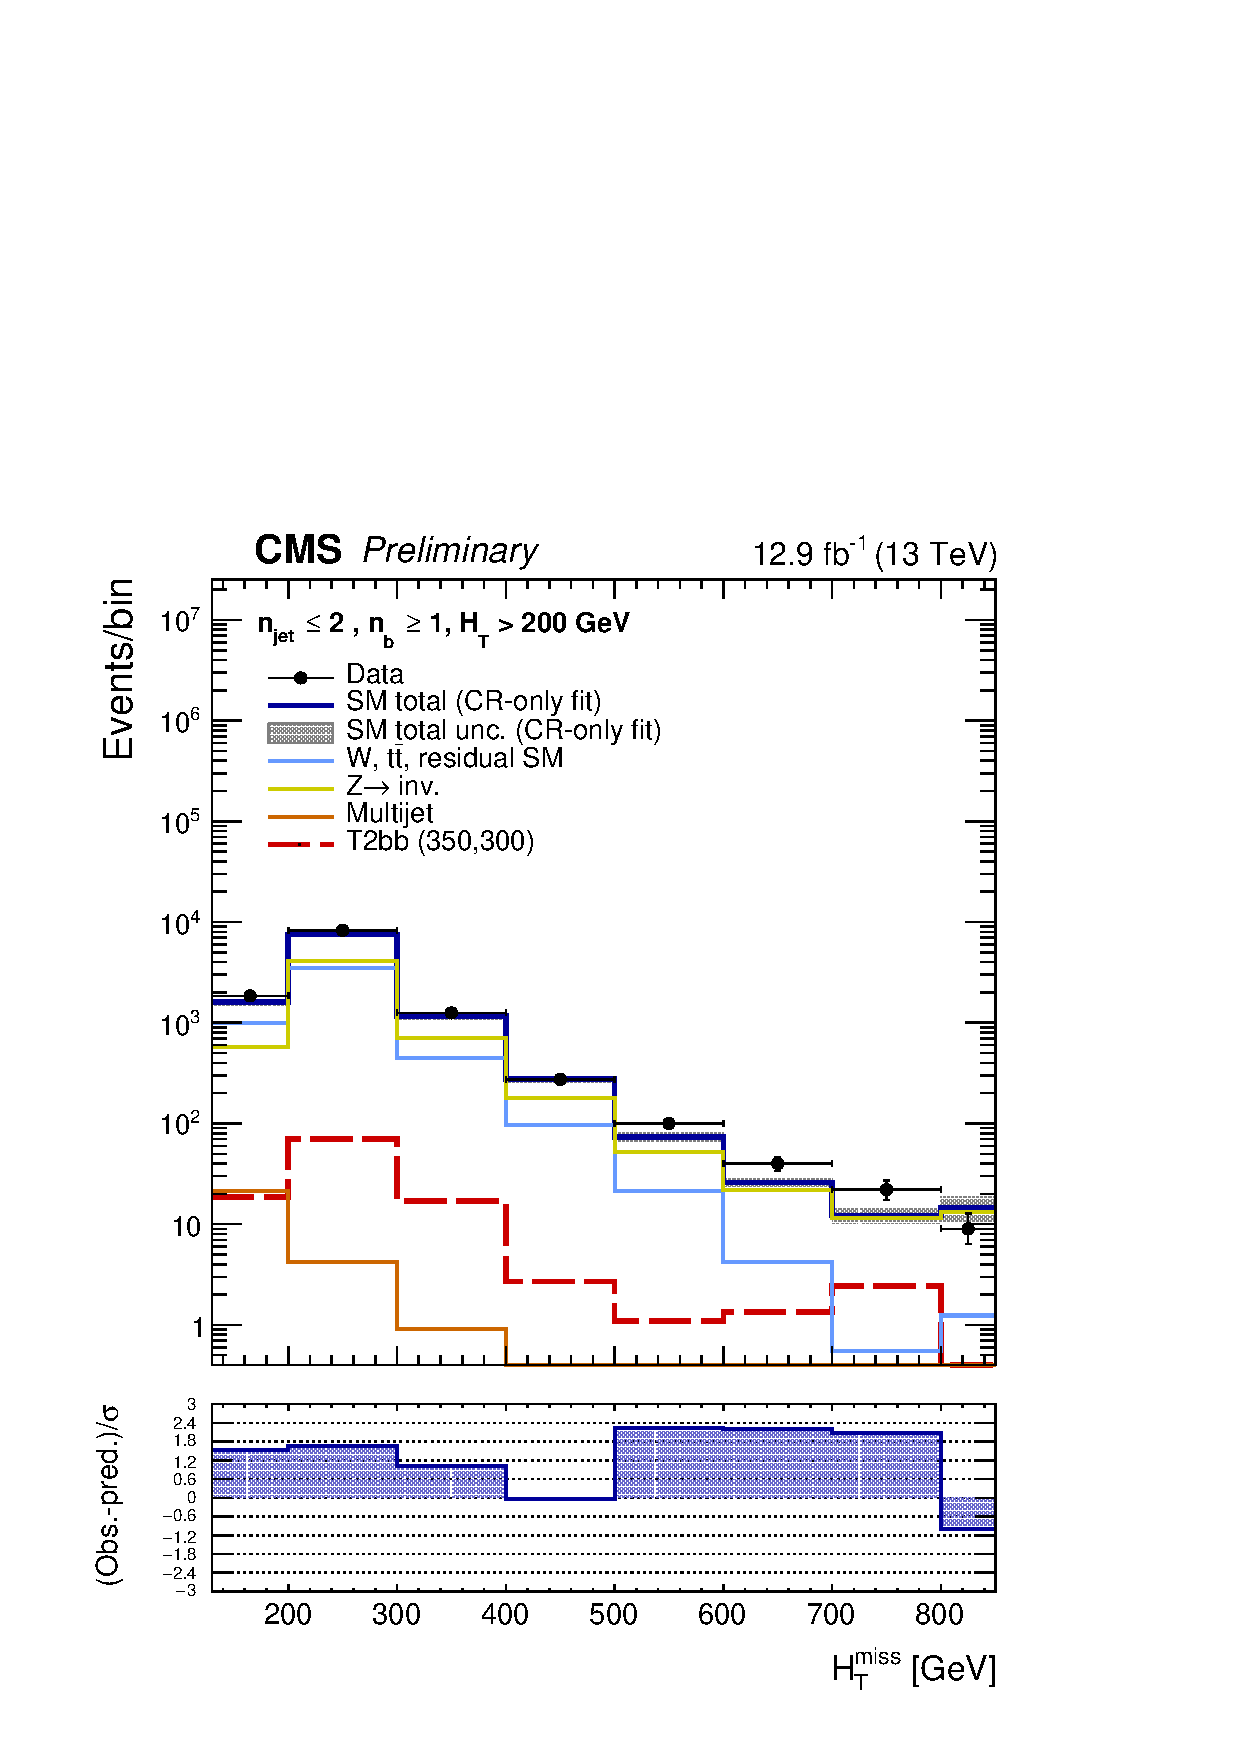
\includegraphics[width=0.4\textwidth]{figures/agg_fitResults/mhtShape_ge1b_le2j_200_Inf_crfit_aux.pdf} } \\
    \subfigure[Asymmetric high \nj, $\nb \leq 1$]   { 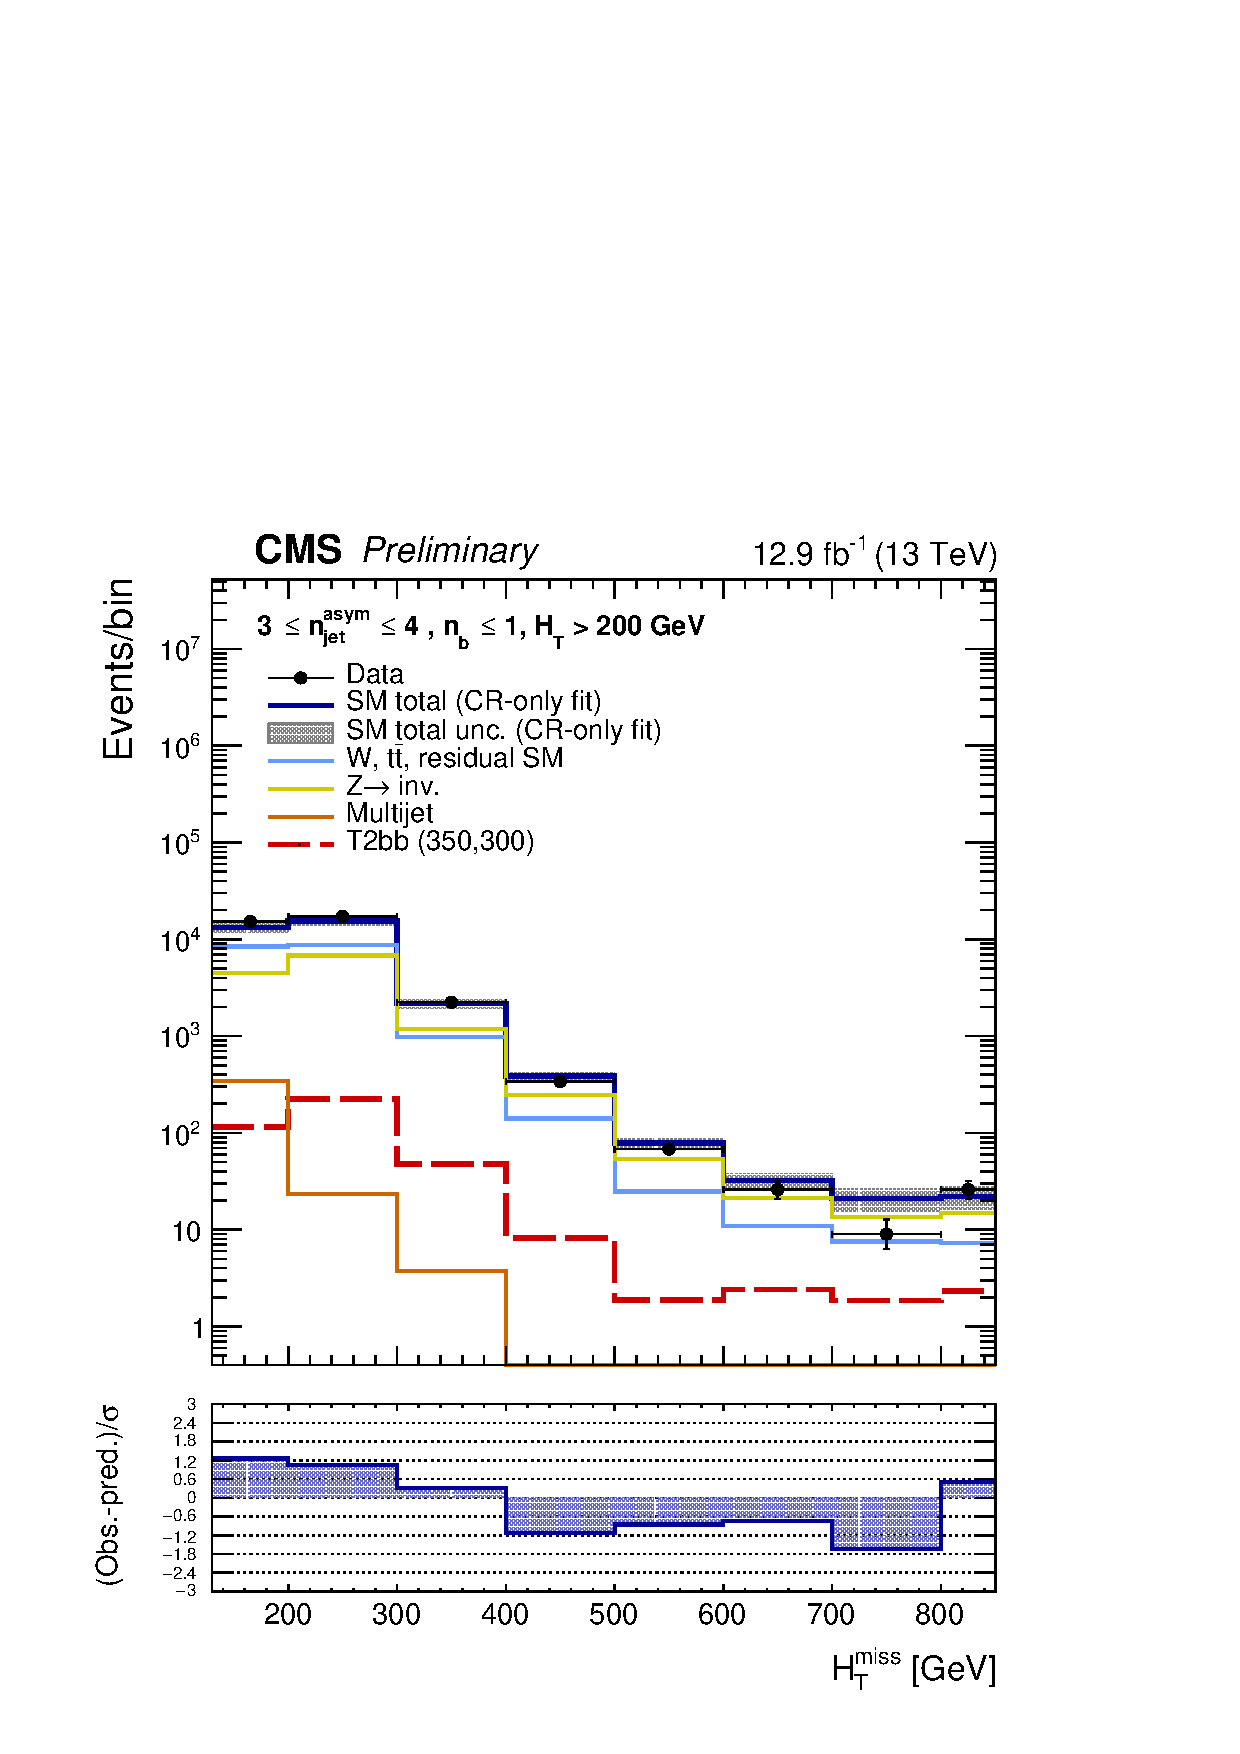
\includegraphics[width=0.4\textwidth]{figures/agg_fitResults/mhtShape_le1b_ge3a_200_Inf_crfit_aux.pdf} } ~~
    \subfigure[Asymmetric high \nj, $\nb \geq 2$]{ 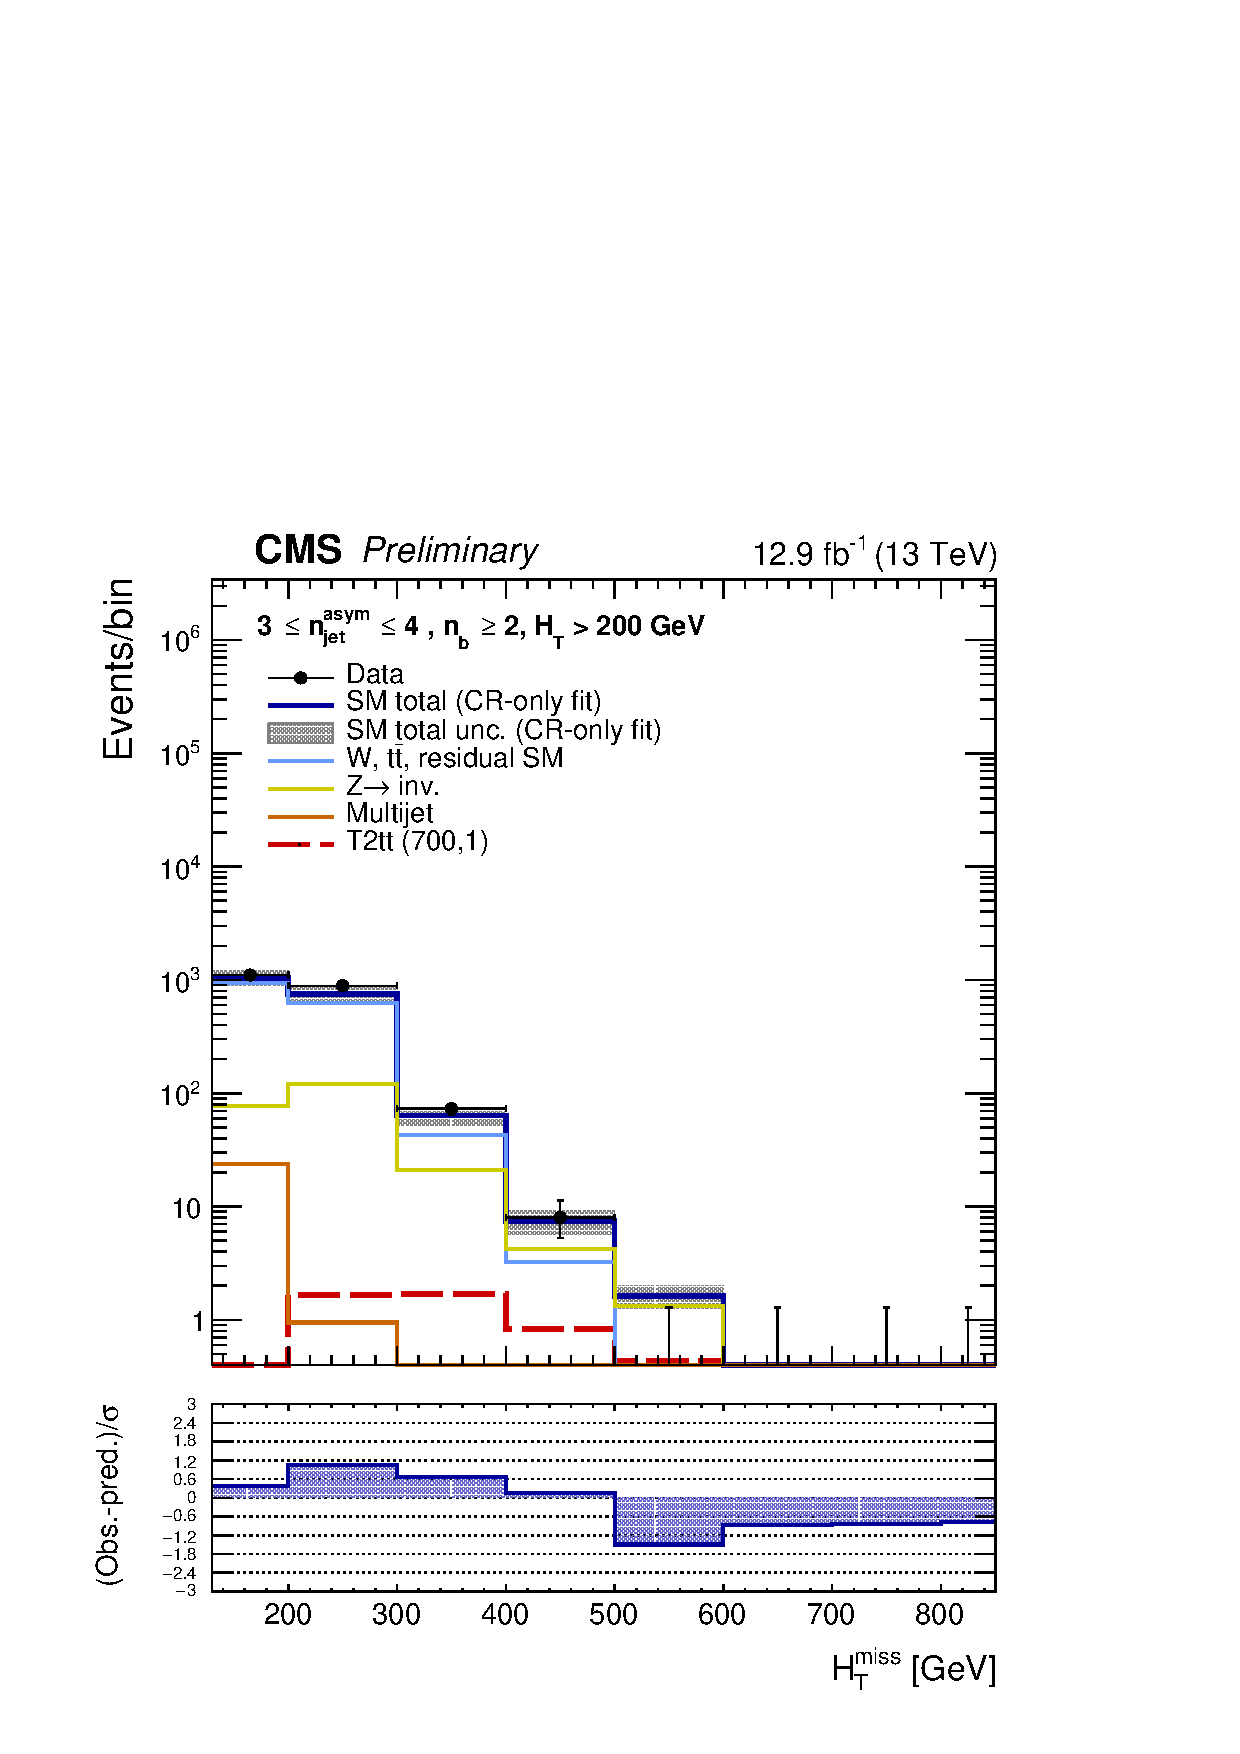
\includegraphics[width=0.4\textwidth]{figures/agg_fitResults/mhtShape_ge2b_ge3a_200_Inf_crfit_aux.pdf} } \\
    \subfigure[Mid \nj, $\nb \leq 1$]   { 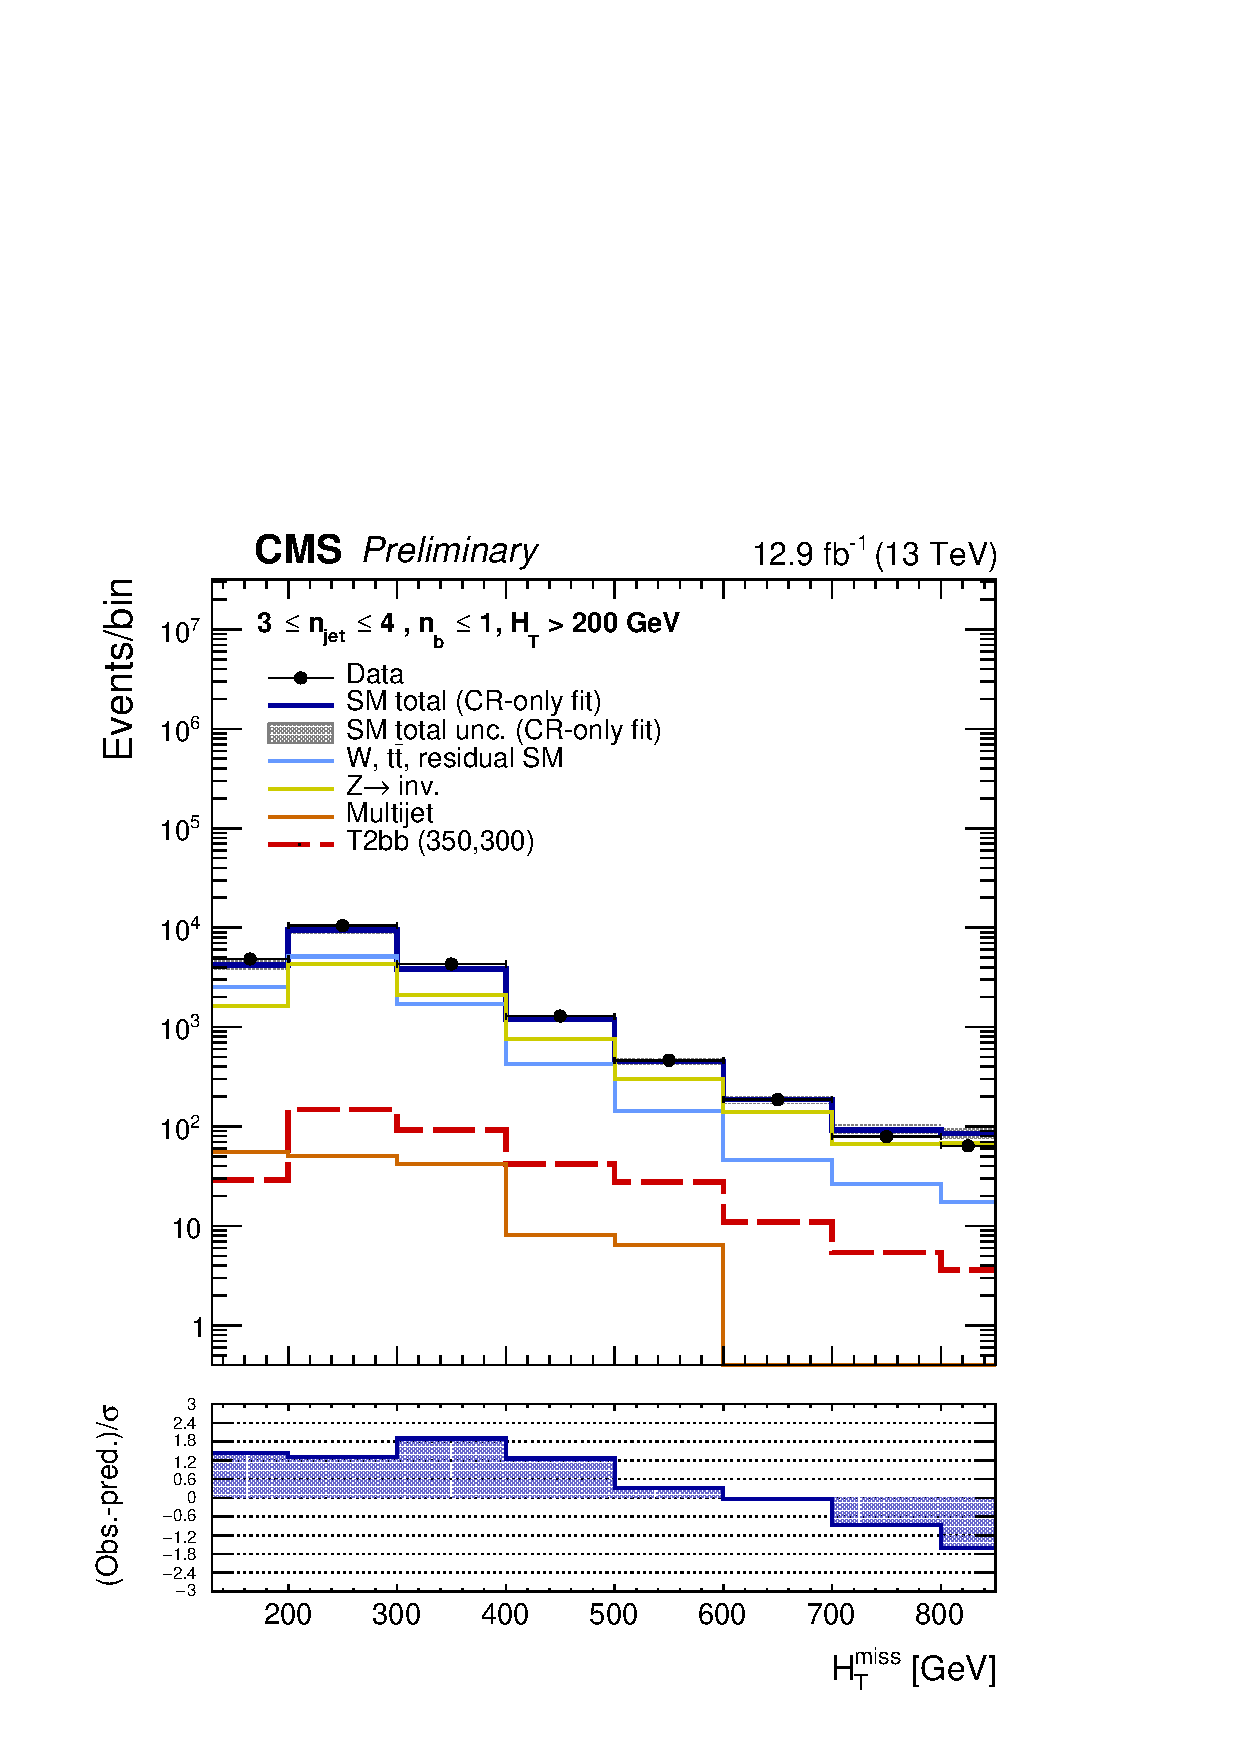
\includegraphics[width=0.4\textwidth]{figures/agg_fitResults/mhtShape_le1b_ge3j_200_Inf_crfit_aux.pdf} } ~~
    \subfigure[Mid \nj, $\nb \geq 2$]{ 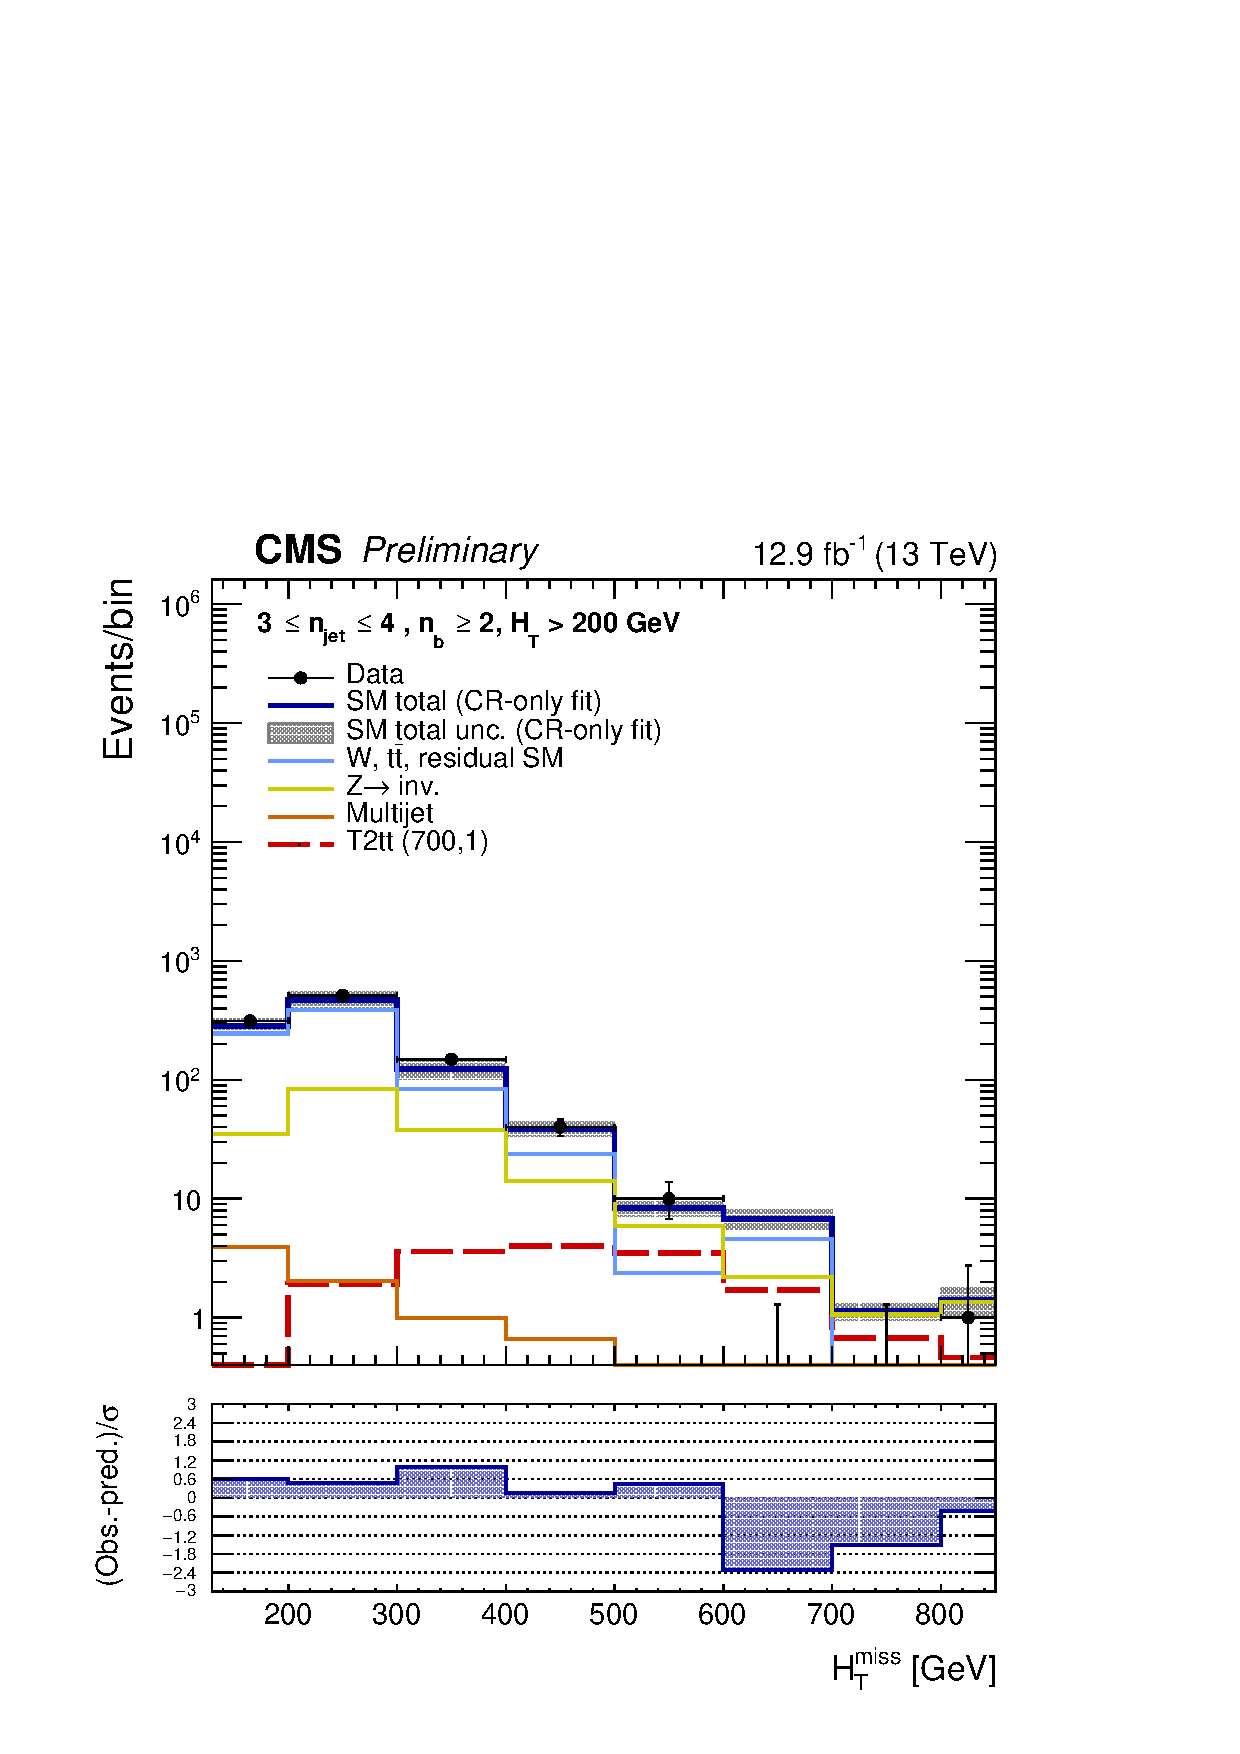
\includegraphics[width=0.4\textwidth]{figures/agg_fitResults/mhtShape_ge2b_ge3j_200_Inf_crfit_aux.pdf} } \\
    \subfigure[High \nj, $\nb \leq 1$]   { 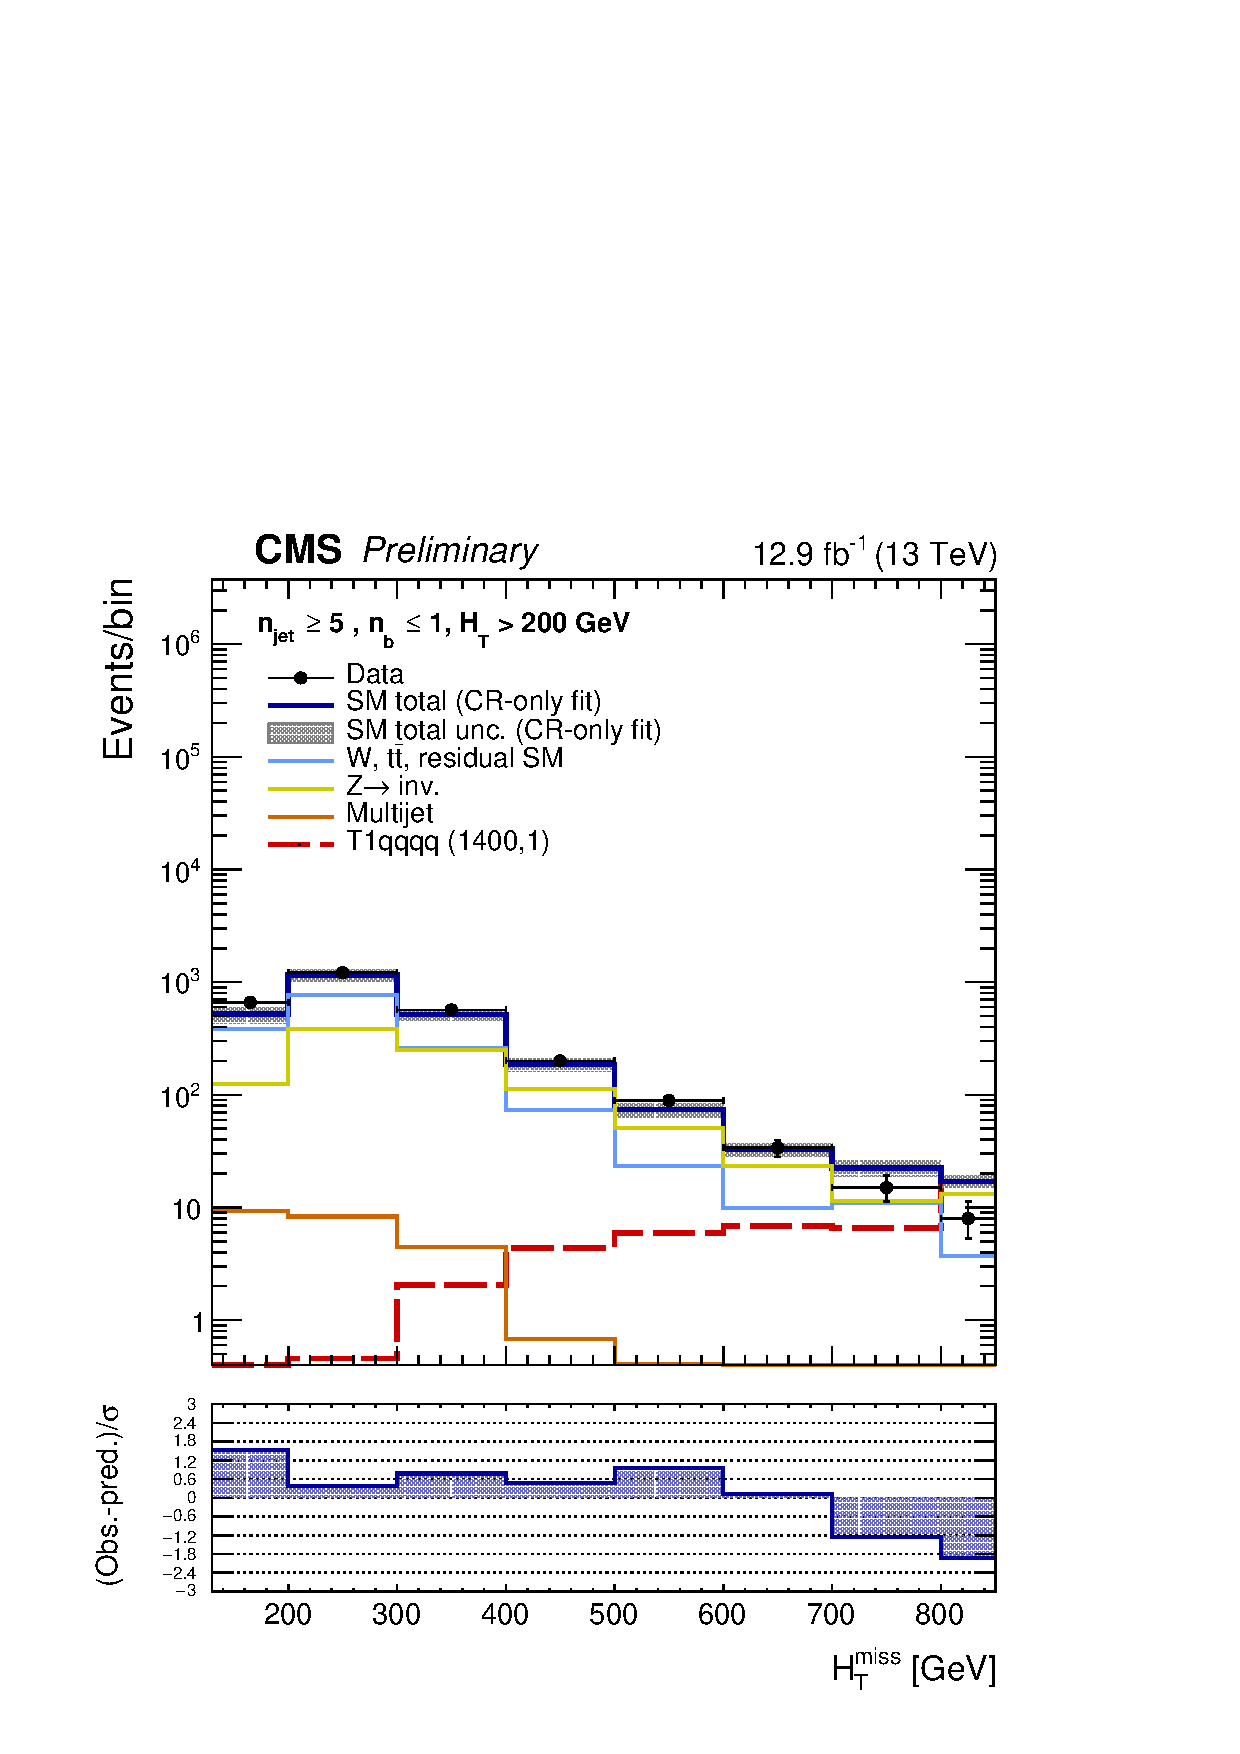
\includegraphics[width=0.4\textwidth]{figures/agg_fitResults/mhtShape_le1b_ge5j_200_Inf_crfit_aux.pdf} } ~~
    \subfigure[High \nj, $\nb \geq 2$]{ 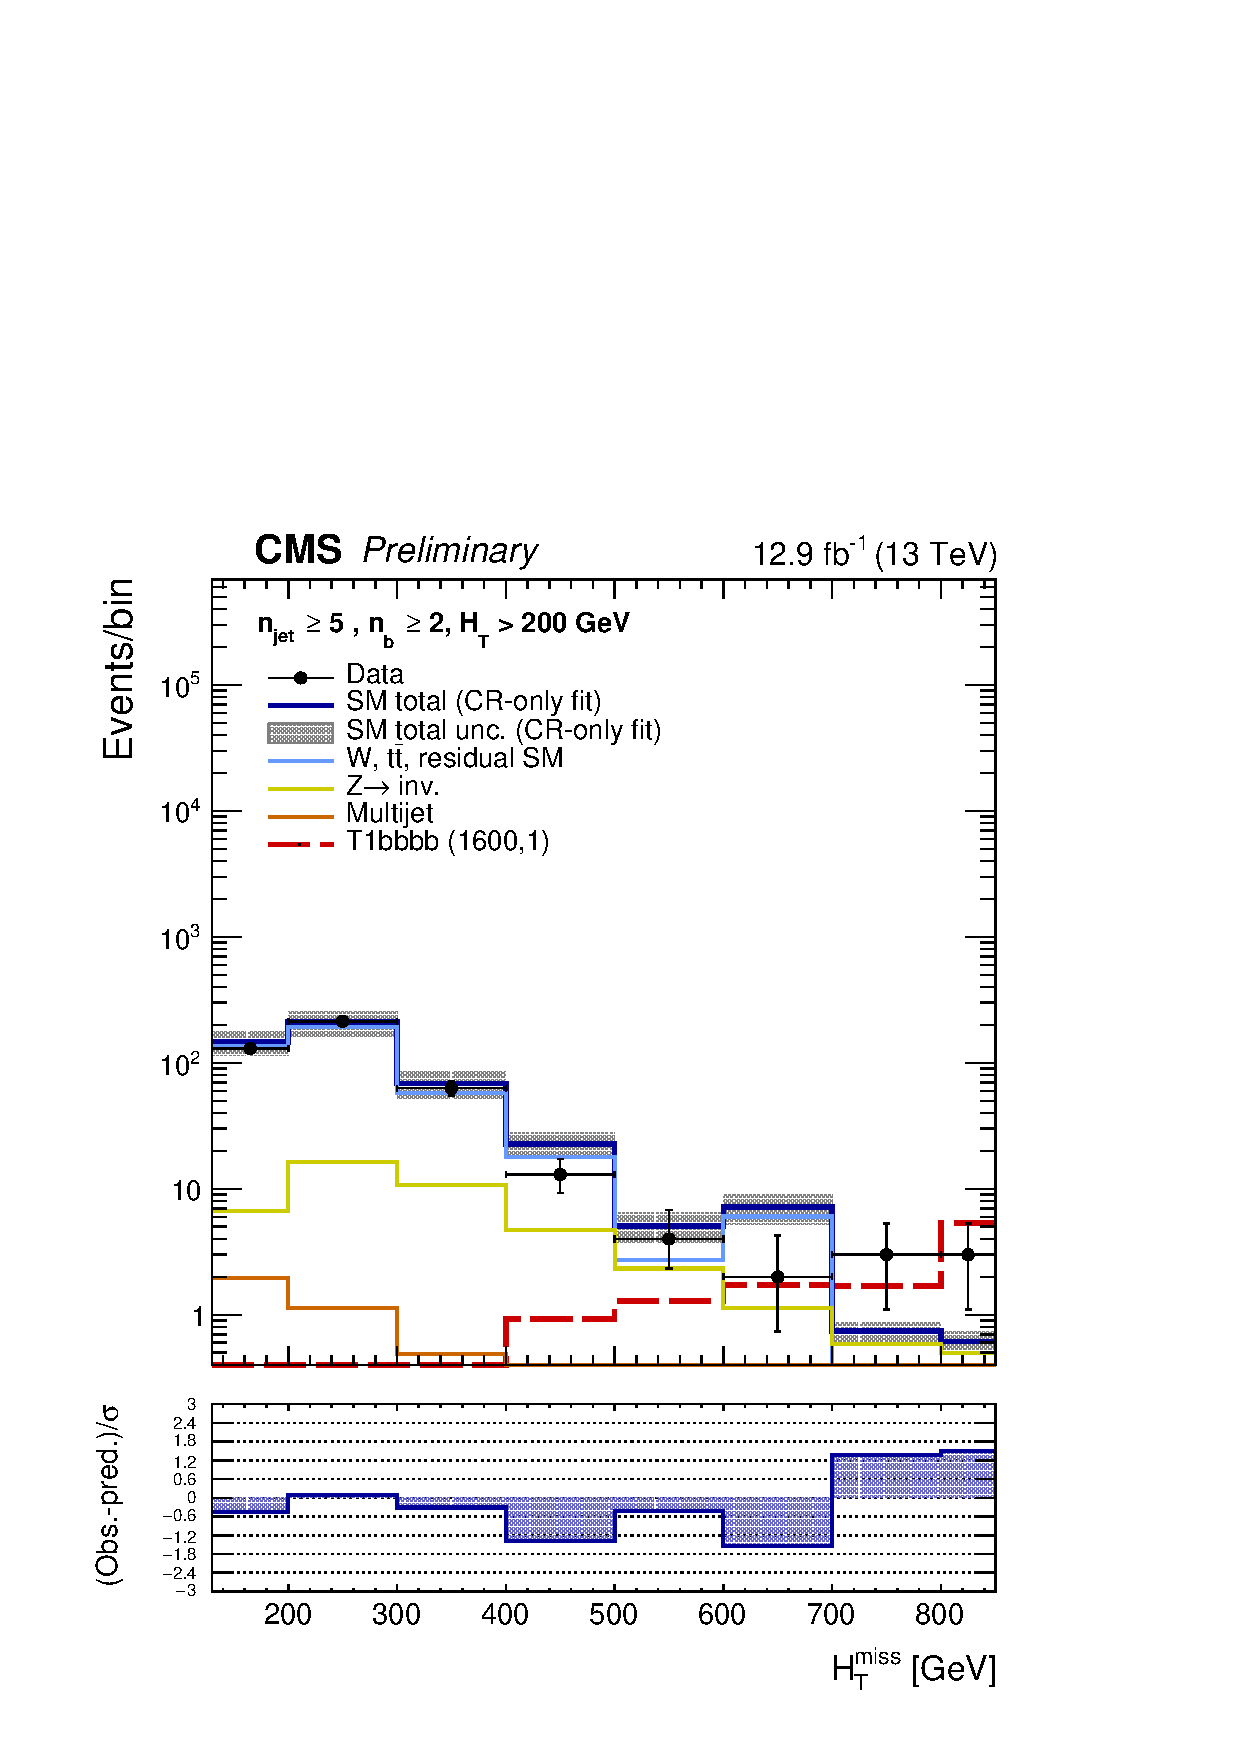
\includegraphics[width=0.4\textwidth]{figures/agg_fitResults/mhtShape_ge2b_ge5j_200_Inf_crfit_aux.pdf} } \\
  \end{center}
\end{figure}


\clearpage
\begin{figure}[!tbhp]
    \caption{ Limit planes shown for both the full signal regions (left) and the aggregate regions (right).\label{fig:limit-planes}. 
    For the compressed models. }
  \begin{center}
    \subfigure[T2bb full signal region]{ 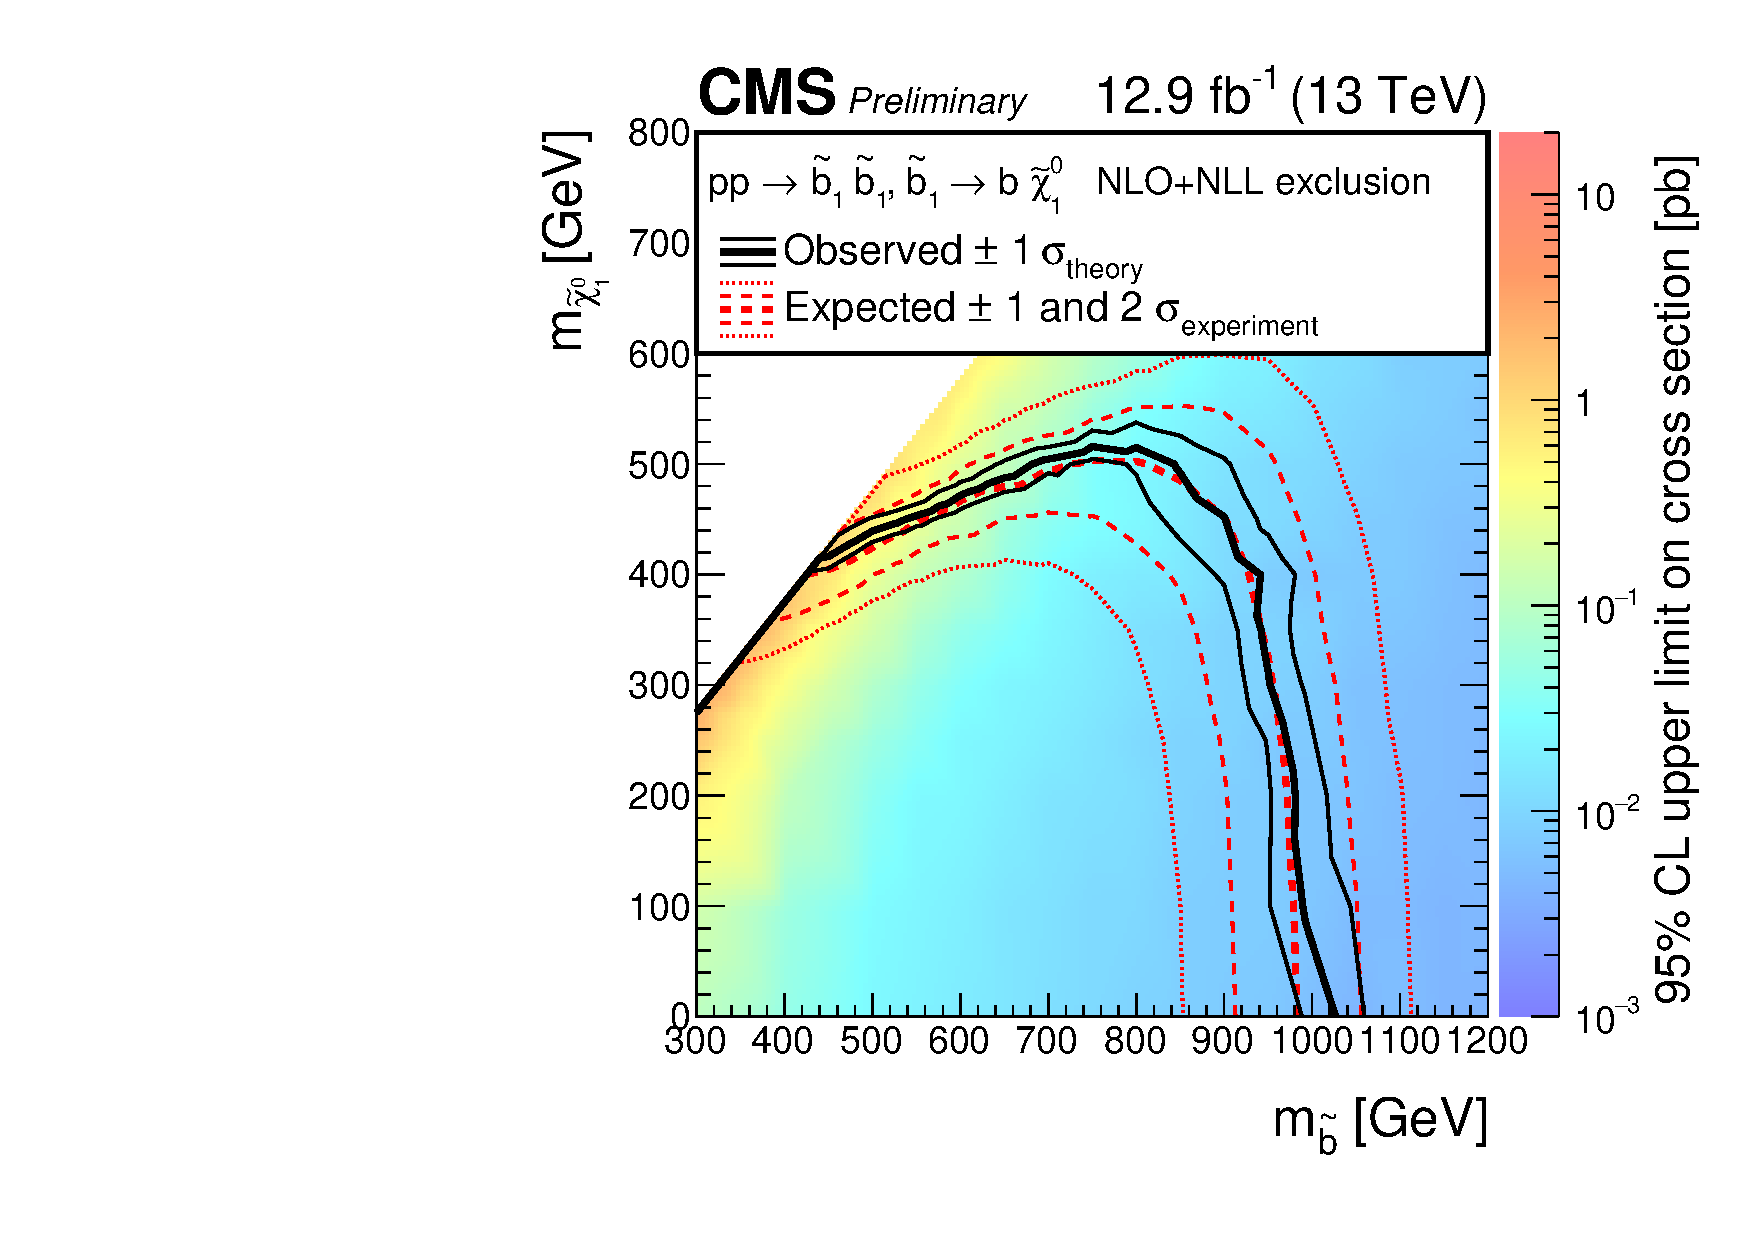
\includegraphics[width=0.45\textwidth]{figures/limitPlanesNominal/SUS16T2bbXSEC} } ~~
    \subfigure[T2bb aggregate regions]{ 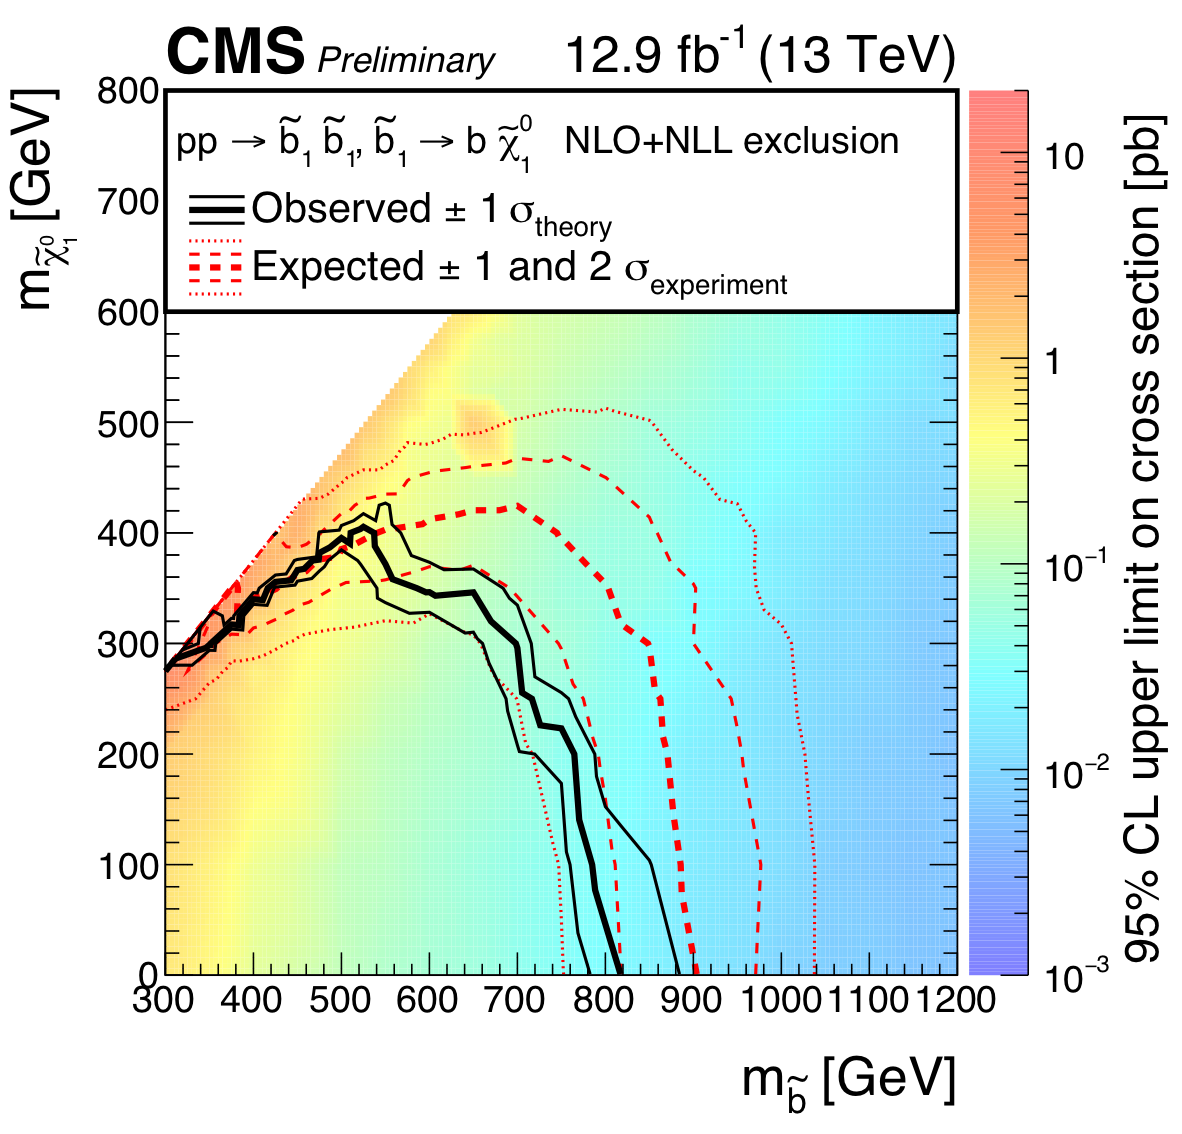
\includegraphics[width=0.45\textwidth]{figures/limitPlanesAgg/SUS16T2bbXSEC} } \\
    \subfigure[T2tt full signal region]   { 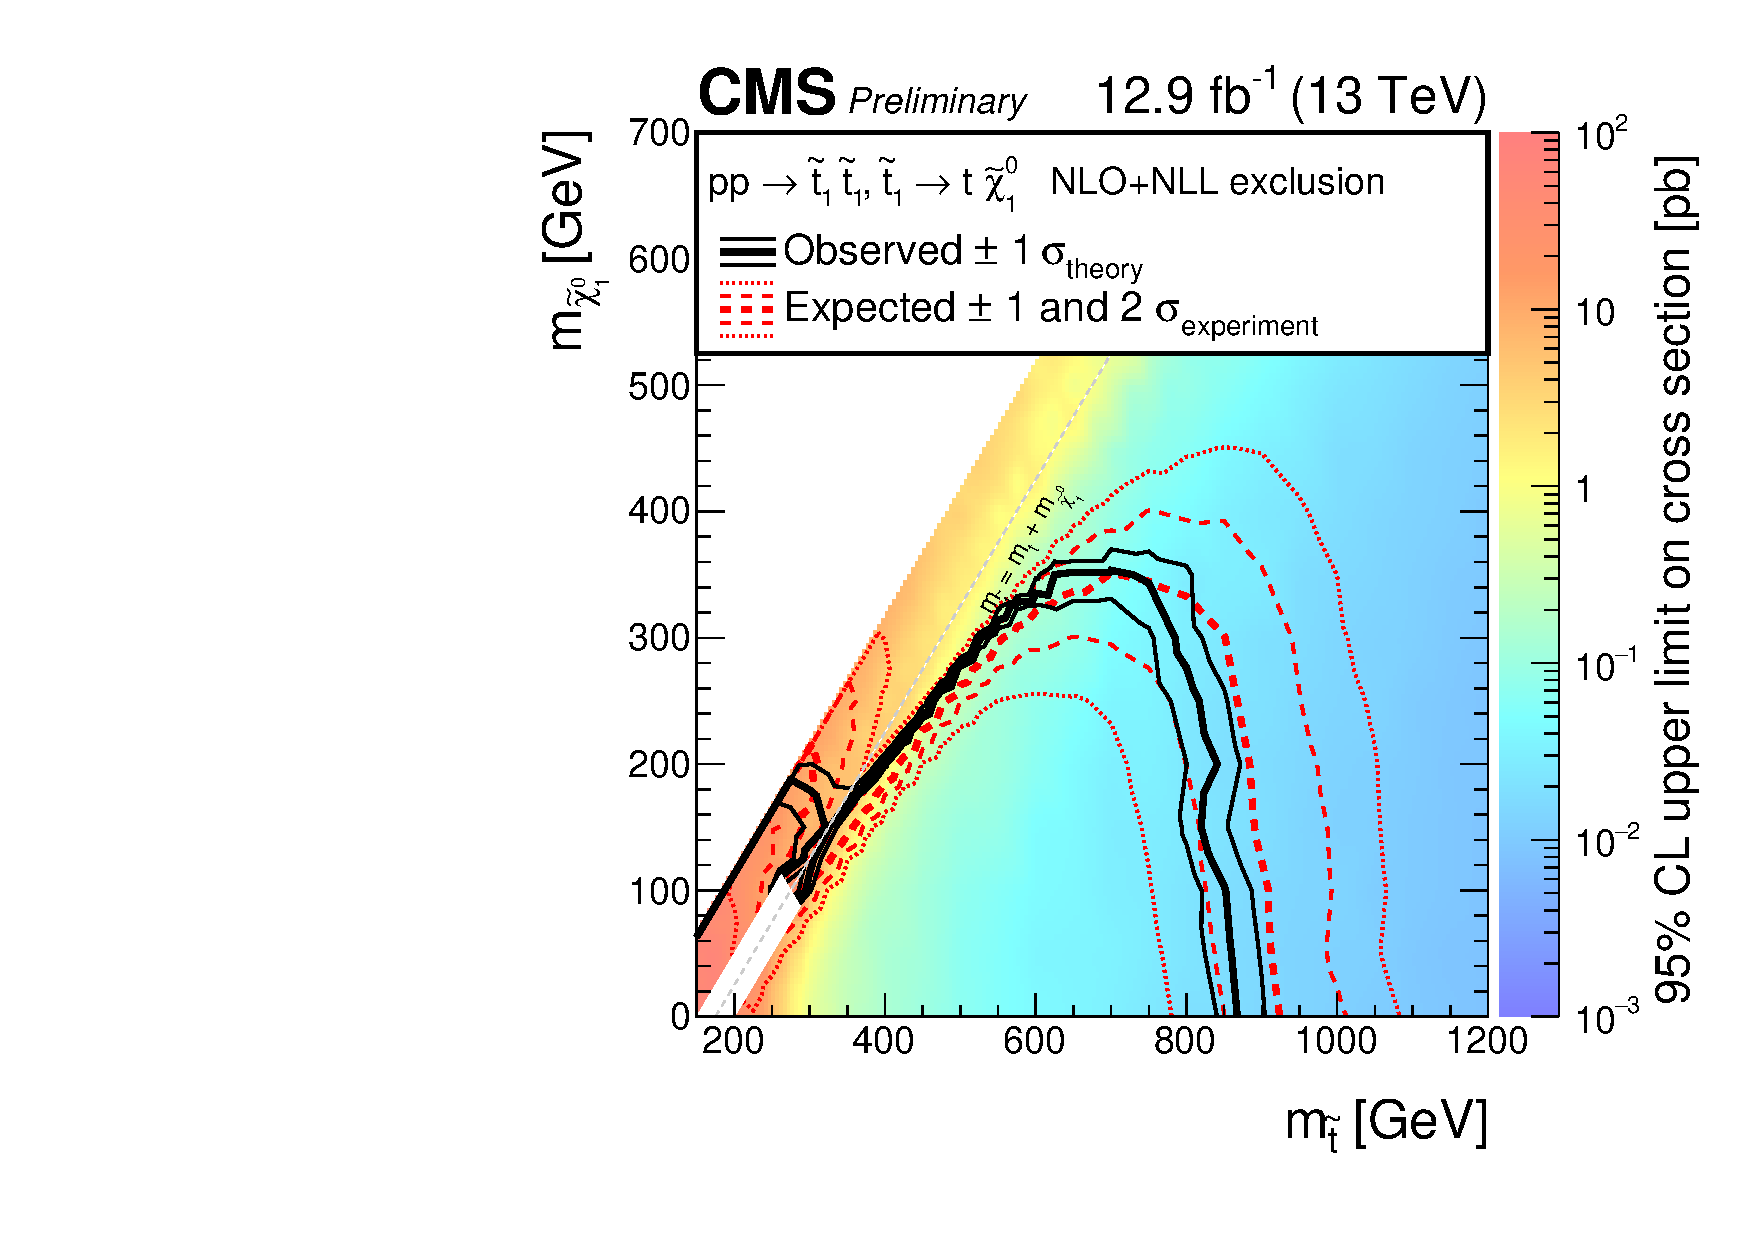
\includegraphics[width=0.45\textwidth]{figures/limitPlanesNominal/SUS16T2ttXSEC} } ~~
    \subfigure[T2tt aggregate regions]{ 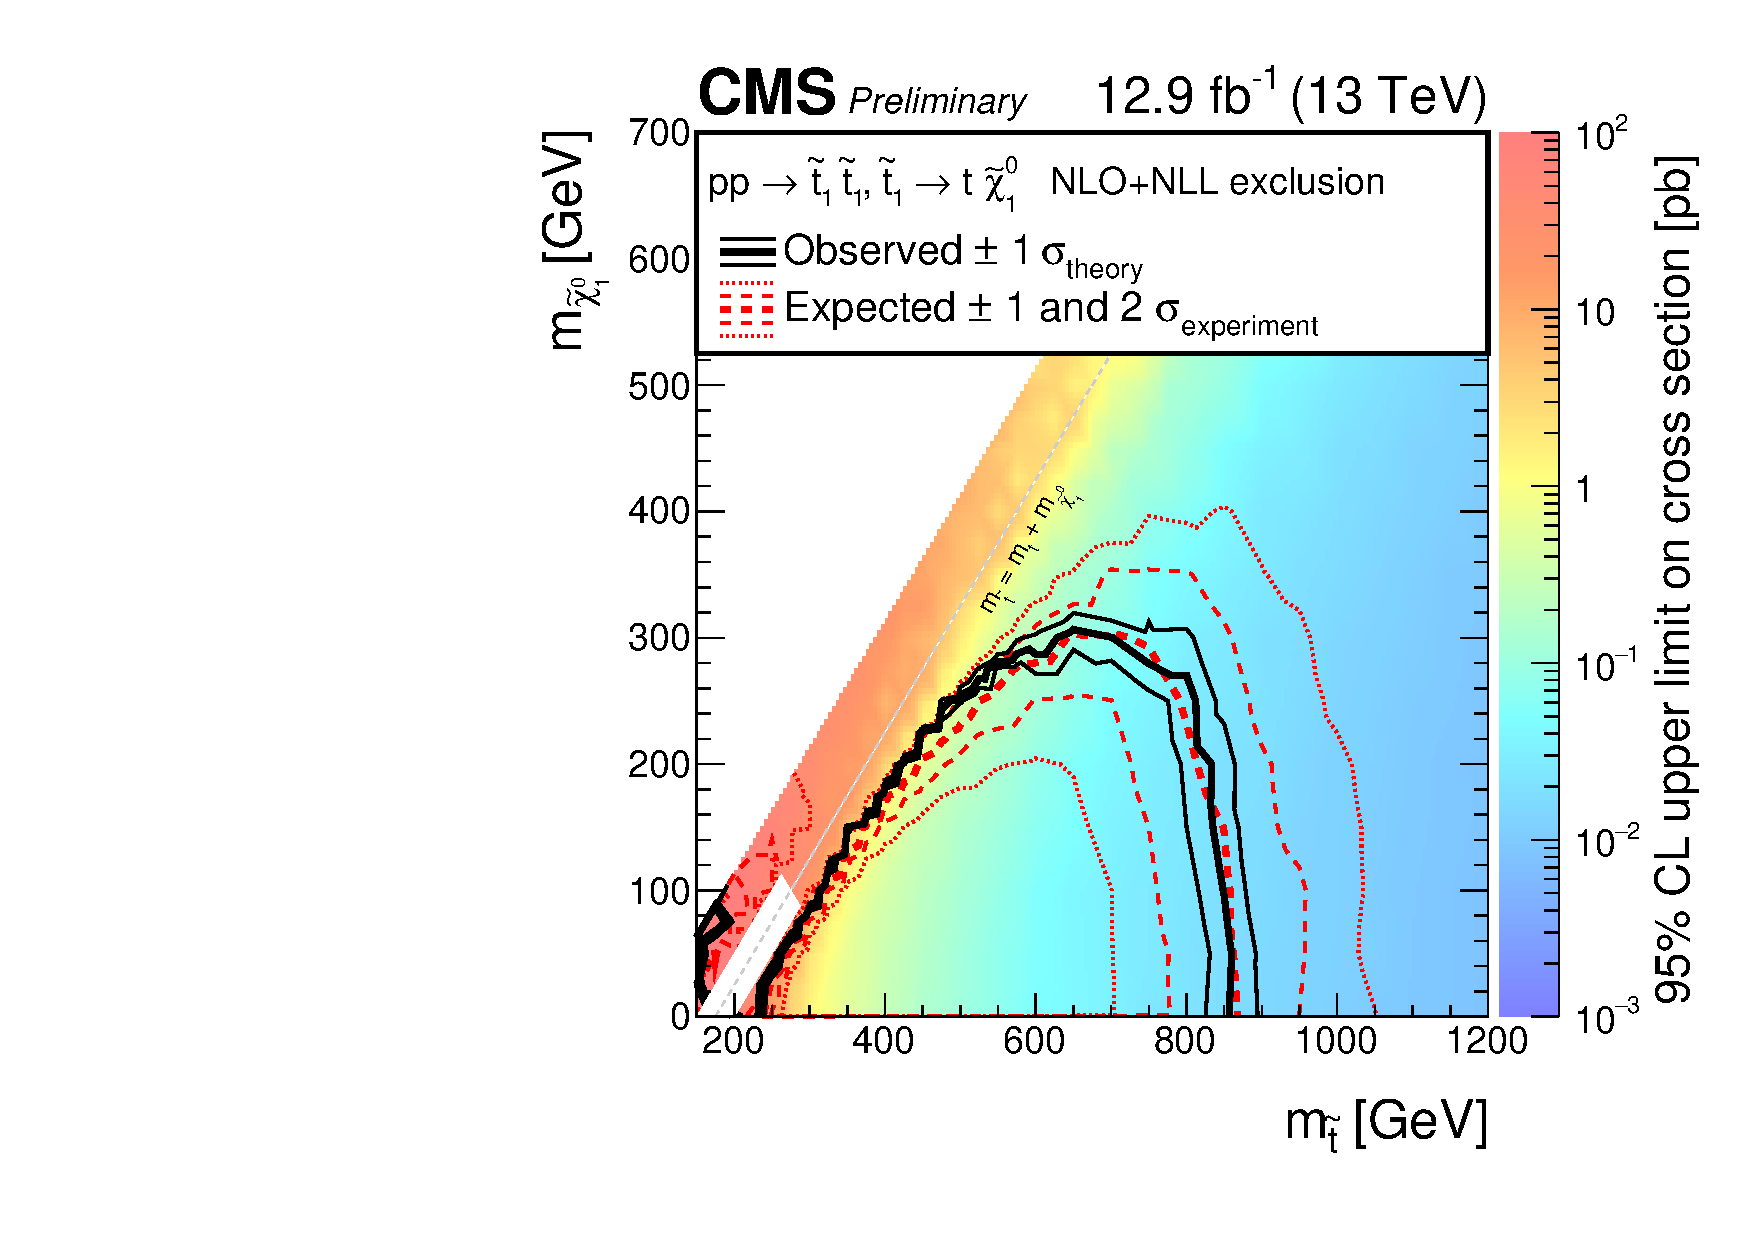
\includegraphics[width=0.45\textwidth]{figures/limitPlanesAgg/SUS16T2ttXSEC} } \\
    \subfigure[T1bbbb full signal region]   { 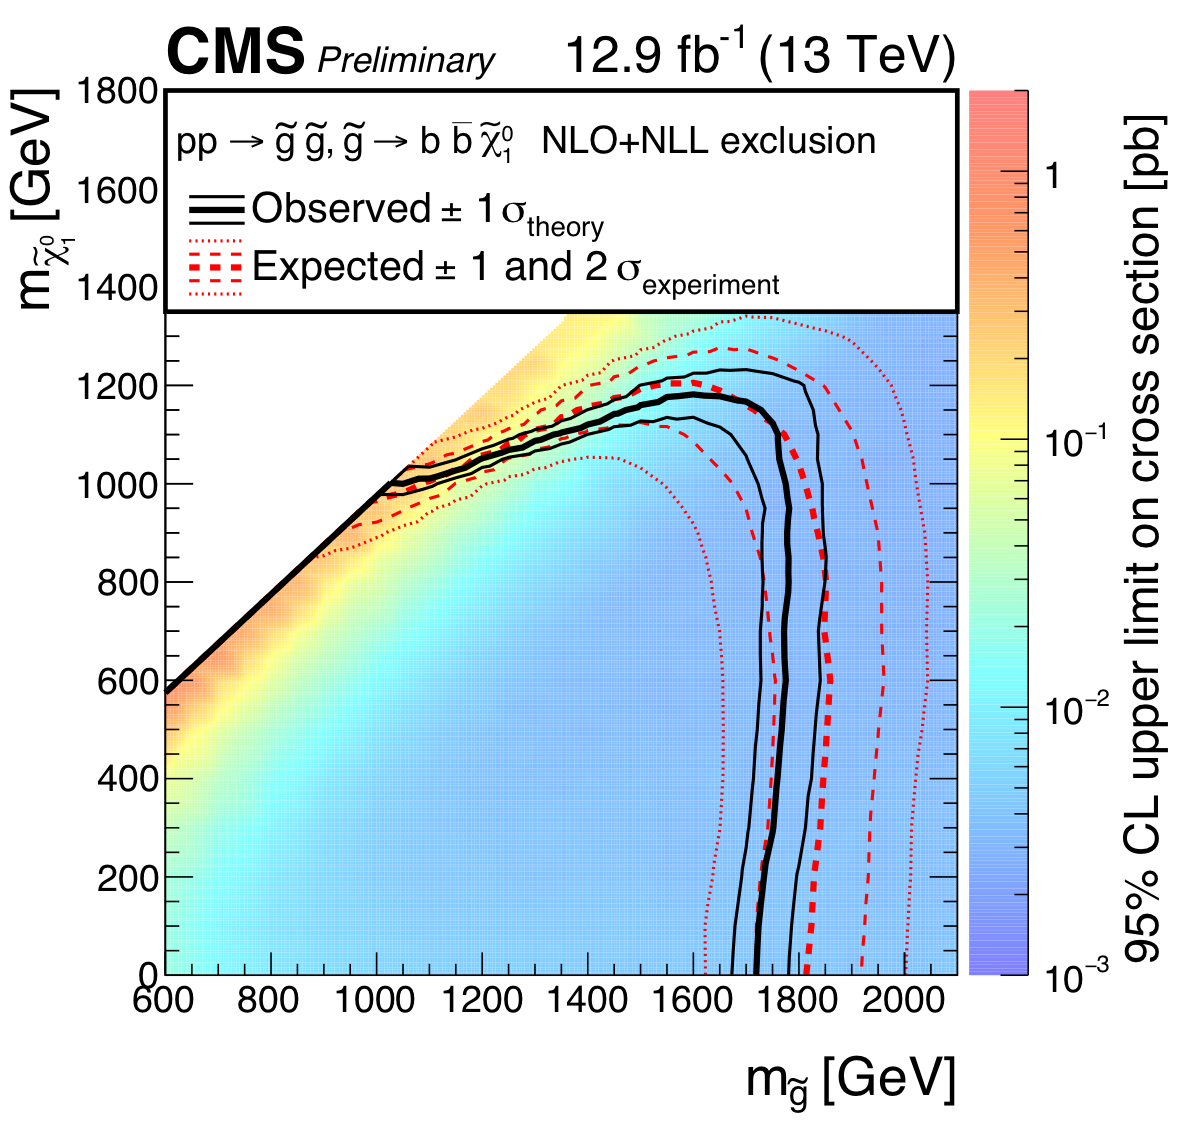
\includegraphics[width=0.45\textwidth]{figures/limitPlanesNominal/SUS16T1bbbbXSEC} } ~~
    \subfigure[T1bbbb aggregate regions]{ 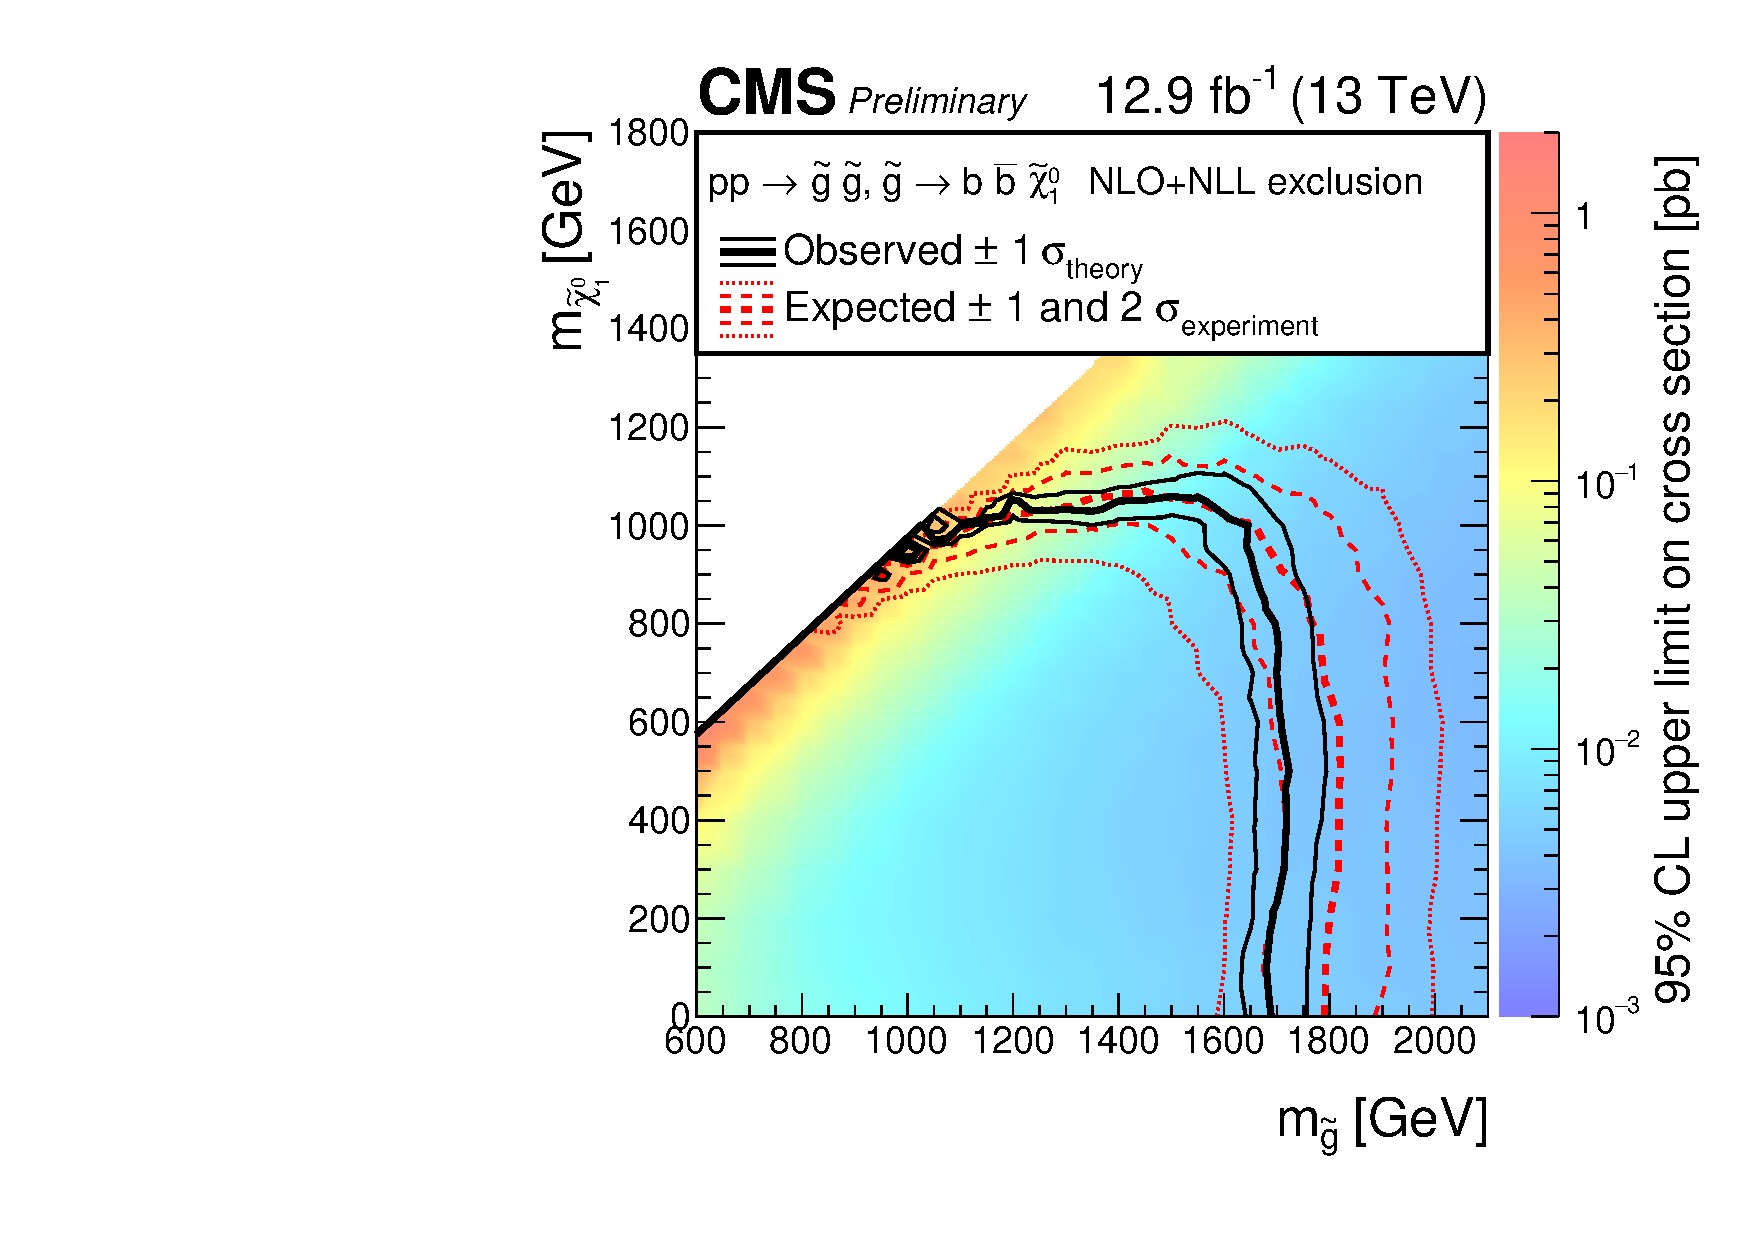
\includegraphics[width=0.45\textwidth]{figures/limitPlanesAgg/SUS16T1bbbbXSEC} } \\
  \end{center}
\end{figure}
%%____________________________________________________________________________||


